\documentclass{standalone}
\begin{document}
	\section{Accuracy}
	
	In this section, I will discuss the results achieved by the implemented pipeline, by comparing these results with the manual annotations (when present)

	To perform the segmentation I have estimated the set of centroids considering $10$ CT scans from the available datasets, carefully selected to achieve a balanced representation for each cluster. The segmentation was performed using as hardware the servers of the Department of Physics and Astronomy(DIFA), and the segmentation of each patient have taken less than $3$ minutes.
	
	\begin{figure}[h!]
		\centering 
		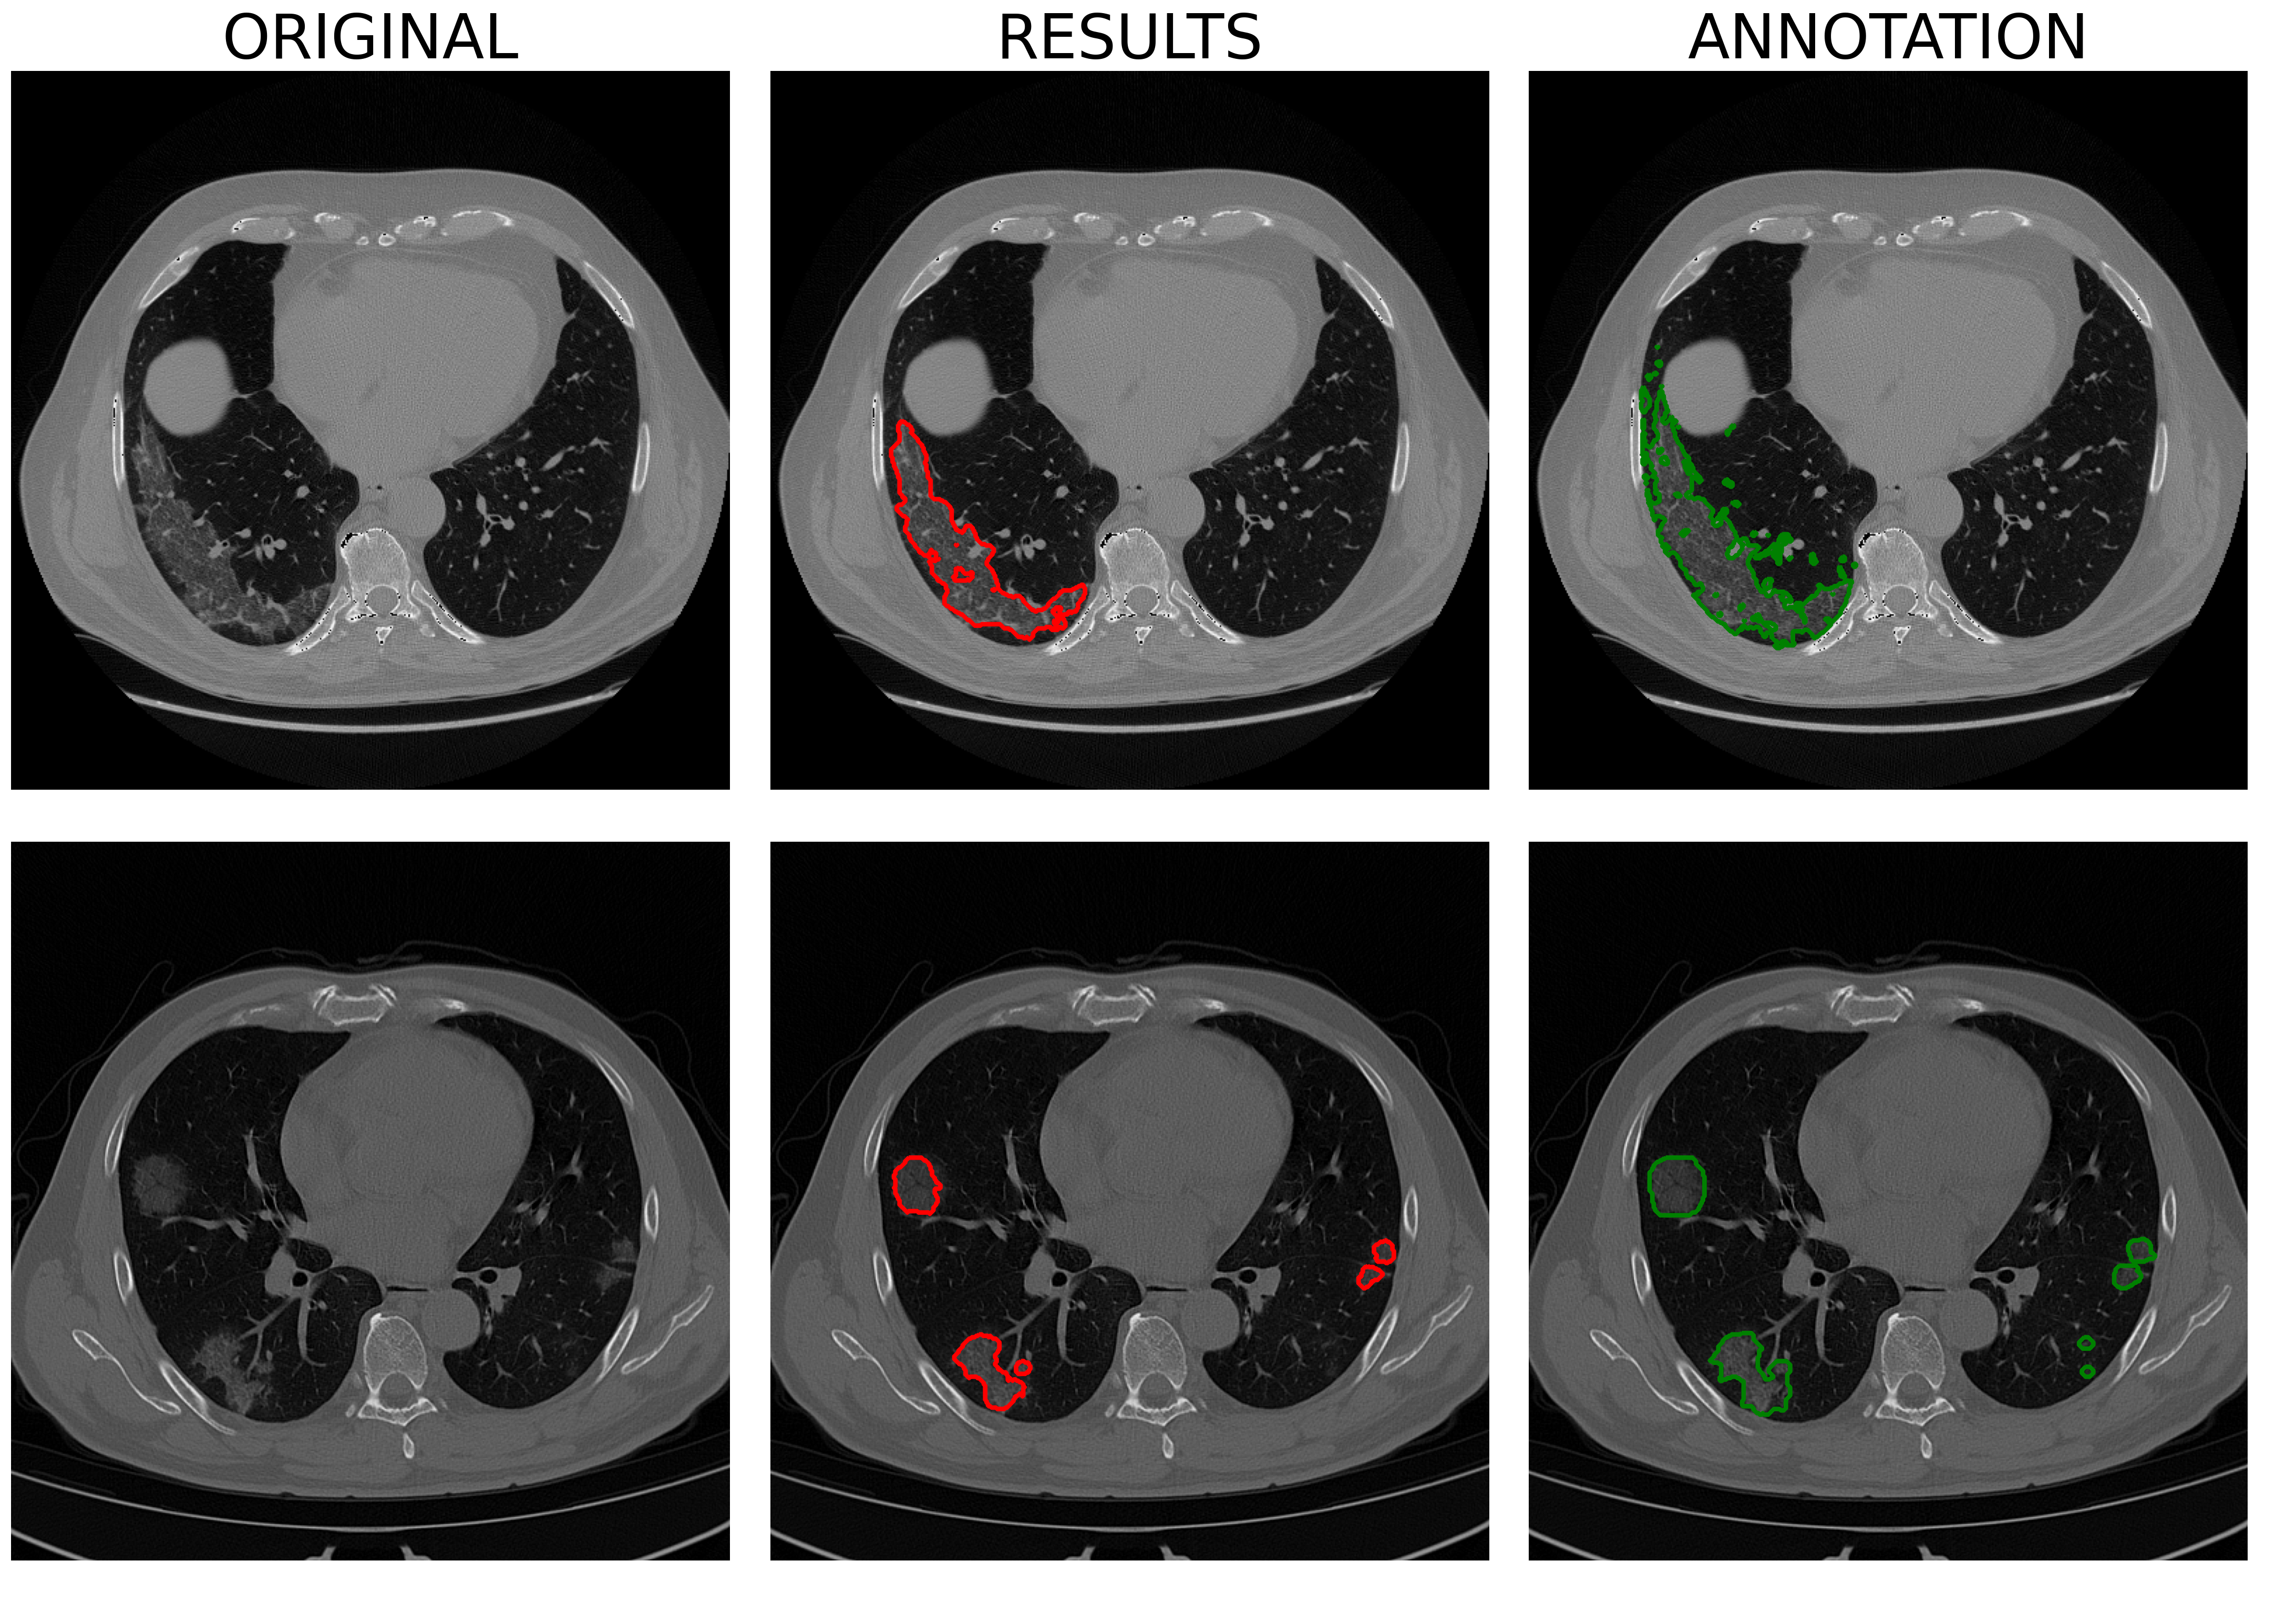
\includegraphics[width=\linewidth]{Results1.png}
		\caption{Comparison between the achieved segmentation (red) and the annotation (green). We clearly see that the GGO and CS areas are well identified and segmented.}\label{fig:Results}
	\end{figure}

	In \figurename\,\ref{fig:Results} I have reported a comparison between the achieved segmentation and the manual annotation as well as the original image. As we can see the lesion areas, seem correctly identified. The resulting segmentation and the annotation seem to be agreement. We can observe that the in, the first case, the annotation find some spots outside the main GGO area. 
	
	\begin{figure}[h!]
		\centering
			\includegraphics[scale=.37]{zoom.png}
		\caption{Focus on the lesion area. From left to right we can observe the original image, the predicted GGO areas and the manual annotation. We can observe that the annotation identify a larger area and also some spots outside the lesions which seems to be healthy tissue.}\label{fig:zoom}
	\end{figure}

	In \figurename\,\ref{fig:zoom} I have provide a zoom on these interesting areas. We can see that the pipeline segmentation well identified the main opacities. We can spot that the annotation tends to consider as GGO a larger region than the pipeline. We can also notice that in the provided annotation also some regions that seem to be healthy are segmented.

	\begin{figure}[h!]	
		\centering 
			\includegraphics[scale=1.1]{3Dlesion.png}
		\caption{3D representation of lung (blue) and identified GGO and CS. From left to right the pipeline segmentation (red) and the manual annotation (green). We can see that the two segmentation seems to agree. The area detected by the pipeline seems to be lower than the manual segmentation.}\label{fig:3Dlabel}		
	\end{figure}
	
	In \figurename\,\ref{fig:3Dlabel} we can see the 3D structure of the lung regions with the identified GGO and CS. In green, we can observe the pipeline results; in pink the manual annotation. As we can see the two regions seem to be consistent. Again we can spot that the annotation tends to consider a larger area than the pipeline.

	I also have matched results and annotation in a quantitative way. Using the $5$ ground truth (accurate and validated manual segmentations) I have matched pipeline and annotation considering sensitivity and specificity.
	Moreover, in collaboration with the Department of Diagnostic and Preventive Medicine of the Policlinico Sant'Orsola - Malpighi, that the segmentation was submitted to five experts in order to make a blind evaluation, comparing the pipeline segmentation with annotation. 
	
\end{document} 